\begin{question}
  \hspace*{\fill} [Note Maximale: 15]\par
  \medskip
  \begin{center} % or flushleft or flushright
    \noindent La figure suivante donne la représentation graphique d'une fonction quadratique $f(x)$, pour $0 \le x \le 4$.\par
    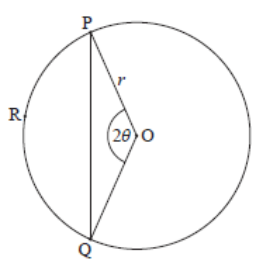
\includegraphics[scale=0.4]{figure_x6}\par
    \noindent La courbe passe par le point $P(0; 13)$, et son sommet est le point $V(2; 1)$.\par
  \end{center} % or flushleft or flushright
  \begin{enumerate}[label=(\alph*)]
    \item La fonction peut s'écrire sous la forme $f(x) = a(x-h)^2 + k$.
      \begin{enumerate}[label=(\roman*)]
        \item Donnez la valeur de $h$ et celle de $k$.
        \item Montrez que $a=3$.\hspace*{\fill} [4]
      \end{enumerate}
    \item Trouvez $f(x)$ et donnez votre réponse sous la forme $Ax^2 + Bx + C$.\hspace*{\fill} [3]
    \item Calculez l'aire délimitée par la courbe de $f$, l’axe des abscisses $Ox$, et les droites $x=2$ et $x=4$.\hspace*{\fill} [8]
  \end{enumerate}
\end{question}
